\documentclass[10pt,a4paper,titlepage]{article}
\usepackage[latin1]{inputenc}
\usepackage[english]{babel}
\usepackage[margin=1.2in]{geometry}
\usepackage{amsmath}
\usepackage{amsfonts}
\usepackage{amssymb}
\usepackage{makeidx}
\usepackage{graphicx}
\usepackage{float}
\usepackage[justification=centering]{caption}
\renewcommand{\labelitemi}{$\bullet$}
\author{Wim Boes \& Robbe Van Rompaey}
\title{LSTM LANGUAGE MODELING\\Experiments on training parameters}
\date{October 22, 2016}
\begin{document}

\maketitle	

\setcounter{tocdepth}{2}
\tableofcontents

\newpage

\section{Introduction}

\subsection{Setup of experiments}
\label{sec:setup}

The purpose of these experiments is to investigate the impact of the different training parameters involved when using recurrent neural networks for language modeling. To this end, the TensorFlow tutorial model of a recurrent neural network for language modeling (publicly available) is used with the Penn Tree Bank dataset for training, validation and testing of the model \cite{tensorflow}.\\
\\
The TensorFlow tutorial language model consists of different parts. The input words, represented by word IDs (integers) unique to each word, are first embedded into multidimensional representations. These are then sequentially fed into a recurrent neural network that consists of layers of LSTM cells \cite{LSTM}. The outputs of this neural network are then turned into a probability vector by a softmax classifier. Each element of this vector is the probability that the next word is the word whose word ID is the index of the element in this vector.\\
\\
This language model uses the Penn TreeBank (PTB) dataset, a popular benchmark for language models \cite{PTB}. This dataset has a vocabulary of 10000 words and is split into train, validation and test sets. It is a relatively small dataset. Out-of-vocabulary words are mapped to a special $<$unk$>$-token that is also a part of the vocabulary.

\subsection{Explanation of training parameters}
\label{subsec:exp}

This section contains an overview of the different training parameters that will be referenced throughout the rest of this document. These training parameters can be changed in the TensorFlow tutorial language model (Python) files. They do not refer to the actual parameters of the model, such as the weights of the neurons in the neural networks.

\subsubsection{init\_scale}
	
All weights of the language model (the weights of the neurons of the neural network, the coefficients of the logistic regression used in the softmax function, etc.) are initialized uniformly in the range $[\textbf{-init\_scale},\textbf{init\_scale}]$.

\subsubsection{learning\_rate}

The parameter \textbf{learning\_rate} indicates the starting learning rate of the optimization algorithm (see also section \ref{subsubsec:opt}).

\subsubsection{max\_grad\_norm}

The gradients calculated by the BackPropagation Through Time algorithm are clipped at a threshold, namely \textbf{max\_grad\_norm}, to prevent the exploding gradients problem \cite{bptt,exp}.

\subsubsection{num\_layers}

As mentioned in section \ref{sec:setup}, the neural network consists of layers of LSTM cells. The parameter \textbf{num\_layers} indicates how many layers are present in the model.

\subsubsection{num\_steps}
\label{subsubsec:numsteps}

The gradients used during training (by the optimization algorithms) are calculated by the BackPropagation Through Time algorithm, in which the the recurrent neural network is unfolded and regarded as a deep network \cite{bptt}. The parameter \textbf{num\_steps} indicates the number of unfolded layers used.

\subsubsection{hidden\_size}

This parameter indicates the number of neurons in each hidden layer.

\subsubsection{max\_epoch}
\label{subsubsec:max}

This is the number of training epochs without learning rate decay. For example, if \textbf{max\_epoch} is 4 and \textbf{max\_max\_epoch} (see section \ref{subsubsec:maxmax}) is 8, the first 4 epochs the optimizer will use the initial learning rate and the last 4 epochs learning rate decay will be applied (see section \ref{subsubsec:decay}).

\subsubsection{max\_max\_epoch}
\label{subsubsec:maxmax}

This parameter indicates the total number of training epochs. This explanation holds as long as early stopping is not applied, as is the case in these experiments. If early stopping was used, \textbf{max\_max\_epoch} would be the maximum number of training epochs.

\subsubsection{keep\_prob}

The used neural network uses dropout to prevent overfitting to the training data \cite{dropout}. \textbf{keep\_prob} is the probability of keeping the outputs of each layer (applied to each element of the output separately, not to the output as a whole). The kept outputs are adjusted with a correction factor to conserve the energy in the connection.

\subsubsection{lr\_decay}
\label{subsubsec:decay}

As described in section \ref{subsubsec:max}, after \textbf{max\_epoch} epochs exponential learning rate decay is applied with factor \textbf{lr\_decay}.

\subsubsection{batch\_size}

\textbf{batch\_size} is the number of training examples per batch. One training example contains \textbf{num\_steps} words (see section \ref{subsubsec:numsteps}). After each batch the parameters are updated, so that these are updated mutiple times during one epoch.

\subsubsection{embedded\_size}

As mentioned in section \ref{sec:setup}, the word IDs (integers) are transformed into multidimensional (real-valued) representations called word embeddings. The number of dimensions used is indicated by the parameter \textbf{embedded\_size}.

\subsubsection{optimizer}
\label{subsubsec:opt}

This parameter indicates which optimization algorithm (available in the Tensorflow package) is used to train the model (by minimizing the loss function, see section \ref{subsubsec:loss}) \cite{opt}. The possible values of \textbf{optimizer} are the following:

\begin{itemize}

	\item \textit{"GradDesc"}: gradient descent algorithm.
	\item \textit{"Adadelta"}: Adadelta algorithm, does not use learning rate parameters \textbf{learning\_rate}, \textbf{lr\_decay} and \textbf{max\_epoch}.
	\item \textit{"Adagrad"}: Adagrad algorithm.
	\item \textit{"Momentum"}: Momentum algorithm, with a fixed momentum term of 0.33 (arbitrary value).
	\item \textit{"Adam"}: Adam algorithm, does not use learning rate parameters \textbf{learning\_rate}, \textbf{lr\_decay} and \textbf{max\_epoch}.	

\end{itemize}

\subsubsection{loss\_function}
\label{subsubsec:loss}

This parameter indicates which loss function is used by the optimizer (see section \ref{subsubsec:opt}). There are two options for \textbf{loss\_function}:

\begin{itemize}
	
	\item \textit{``sequence\_loss\_by\_example''}: cross-entropy using full softmax:
	\[ \text{loss} = -\frac{1}{N} \sum_{i=1}^{N} \ln p_{target_{i}} \]
	\noindent
	with $p_{target_{i}}$ the probability indicated by the output of the language model (see section \ref{sec:setup}) on the position of the target word and N the length of the considered text piece (\textbf{num\_steps}). This corresponds to the Shannon-McMillan-Breimann approximation of the cross-entropy of the language model \cite{cross}.
	
	\item \textit{"sampled\_softmax"}: same loss function as above with some modifications. For the above loss function, for each target word the probability of every word in the vocabulary needs to be computed to obtain  the properly normalized probability $p_{target_{i}}$. For vocabularies that are large, this is impractical. Hence, this loss function samples the vocabulary (32 samples in this case) to compute an approximation of the properly normalized $p_{target_{i}}$, this speeds up training. This loss function can only be used during training, not during inference (because the probability is not properly normalized) \cite{sampled}.
	
\end{itemize}

\section{Results and conclusions of experiments}
\label{sec:results}

This section contains the results and conclusions of the different experiments as described in section \ref{subsec:perf}. As mentioned there, the names of the subsections in this section refer to the variable parameters of the experiment. Each figure shows the different values of the variable parameters as well as the values of the fixed parameters.\\
\\
Some of the figures display the test/validation perplexity as a function of the number of training epochs. The (average-per-word) test/validation perplexity is equal to the exponential value of the average negative log probability (cross-entropy) of the target (test/validation) words:

\[ e^{-\frac{1}{N} \sum_{i=1}^{N} \ln p_{target_{i}}} \]

\noindent
Some of the figures display a bar chart containing the training speed in function of the values of the variable parameters. This speed is expressed in words per seconds.

\subsection{Performed experiments}
\label{subsec:perf}

In this section, the list of performed experiments is given. In each experiment, one or more parameters are variable while the rest of the parameters stay fixed. The next list indicates the variable parameters of each experiment:

\begin{itemize}
	
	\item \textbf{hidden\_size} \textbf{\&} \textbf{embedded\_size}
	\item \textbf{init\_scale} \textbf{\&} \textbf{learning\_rate}
	\item \textbf{num\_steps} \textbf{\&} \textbf{batch\_size}
	\item \textbf{loss\_function}
	\item \textbf{optimizer}
	\item \textbf{num\_layers}
	
\end{itemize}

\noindent
The names of the subsections (one subsection for each experiment) in section \ref{sec:results} will refer to these variable parameters.

\subsection{hidden\_size \& embedded\_size}

\begin{figure}[H]
	\begin{center}
		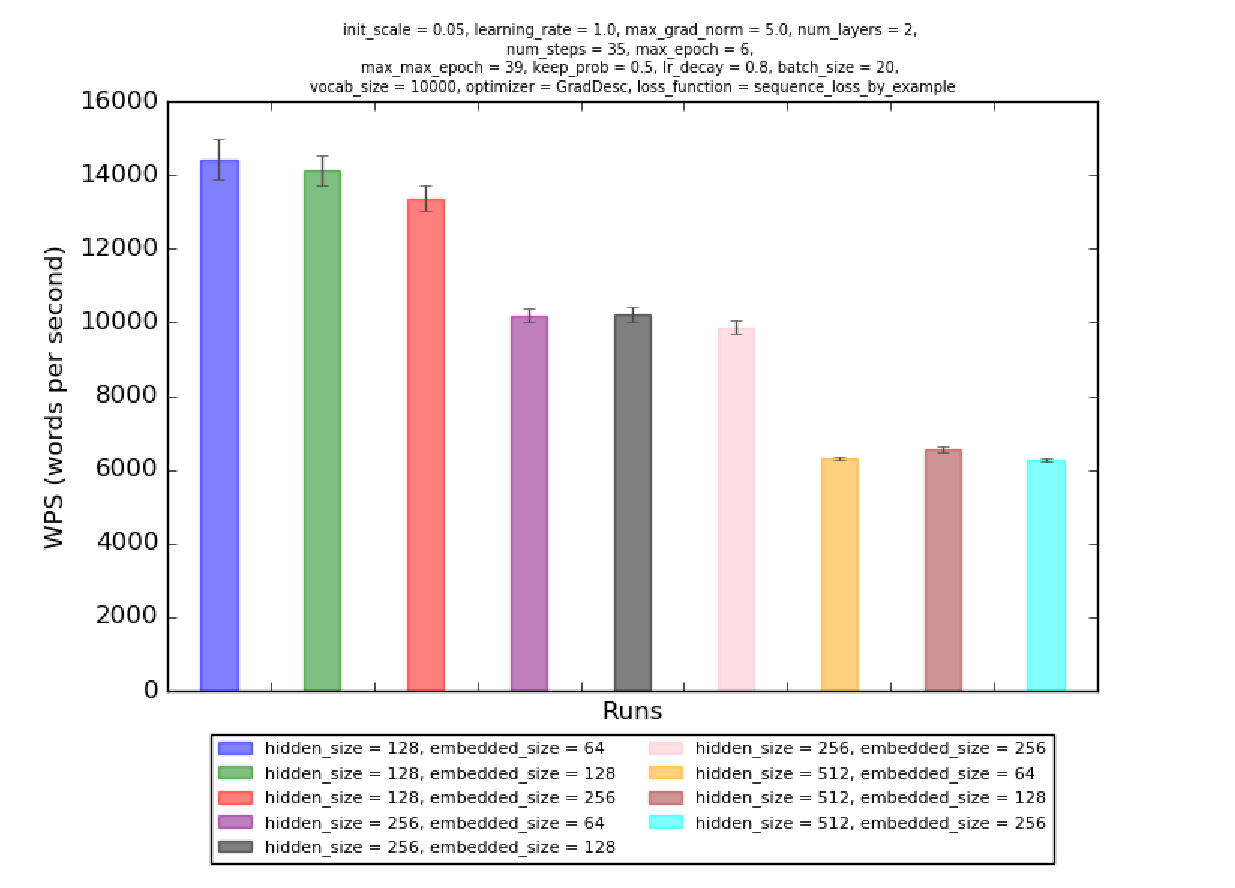
\includegraphics[width=0.70\textwidth]{hidembspeed.eps}
		\caption{Results of speed experiment with \textbf{hidden\_size \& embedded\_size} as variable parameters}
		\label{fig:exp1speed}
	\end{center}	
\end{figure}

\begin{figure}[H]
	\begin{center}
		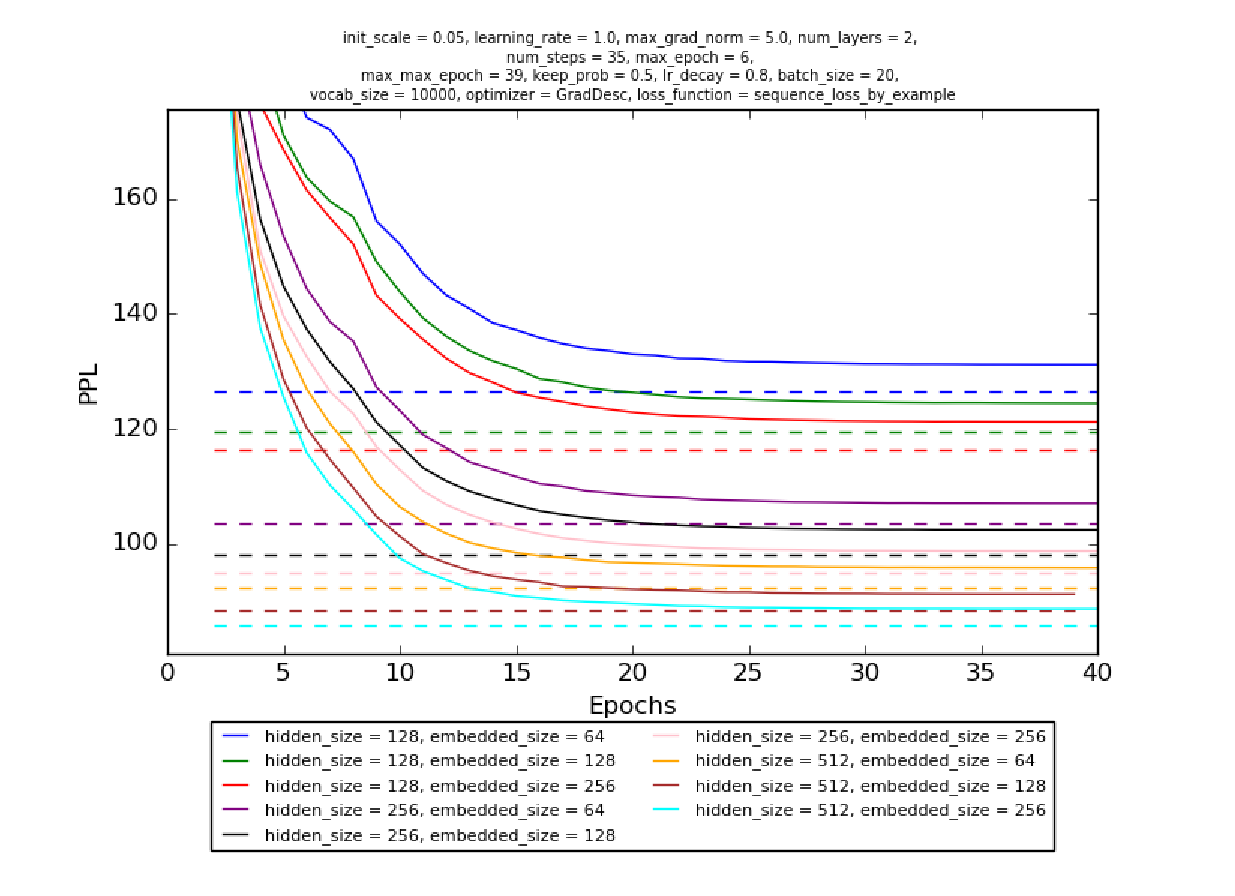
\includegraphics[width=0.70\textwidth]{hidembperf.eps}
		\caption{Results of performance experiment with \textbf{hidden\_size \& embedded\_size} as variable parameters. The full line represents the validation perplexity evaluated after each training epoch, the dotted line represent the test perplexity evaluated at the vary last epoch of the training.}
		\label{fig:exp1perf}
	\end{center}	
\end{figure}

The results of this experiment are displayed in figures \ref{fig:exp1speed} and \ref{fig:exp1perf}. The results are mostly as expected: higher values for \textbf{hidden\_size} generally lead to better performance and slower training speed and higher values for \textbf{embedded\_size} lead to better performance (though less impactful than \textbf{hidden\_size}). However, the parameter \textbf{embedded\_size} does not seem to have a big impact (if any at all) on the training speed. This is interesting as it might suggest that increasing \textbf{embedded\_size} only has positive consequences (at least while the parameter is kept within a certain range).

\subsection{init\_scale \& learning\_rate}

\begin{figure}[H]
	\begin{center}
		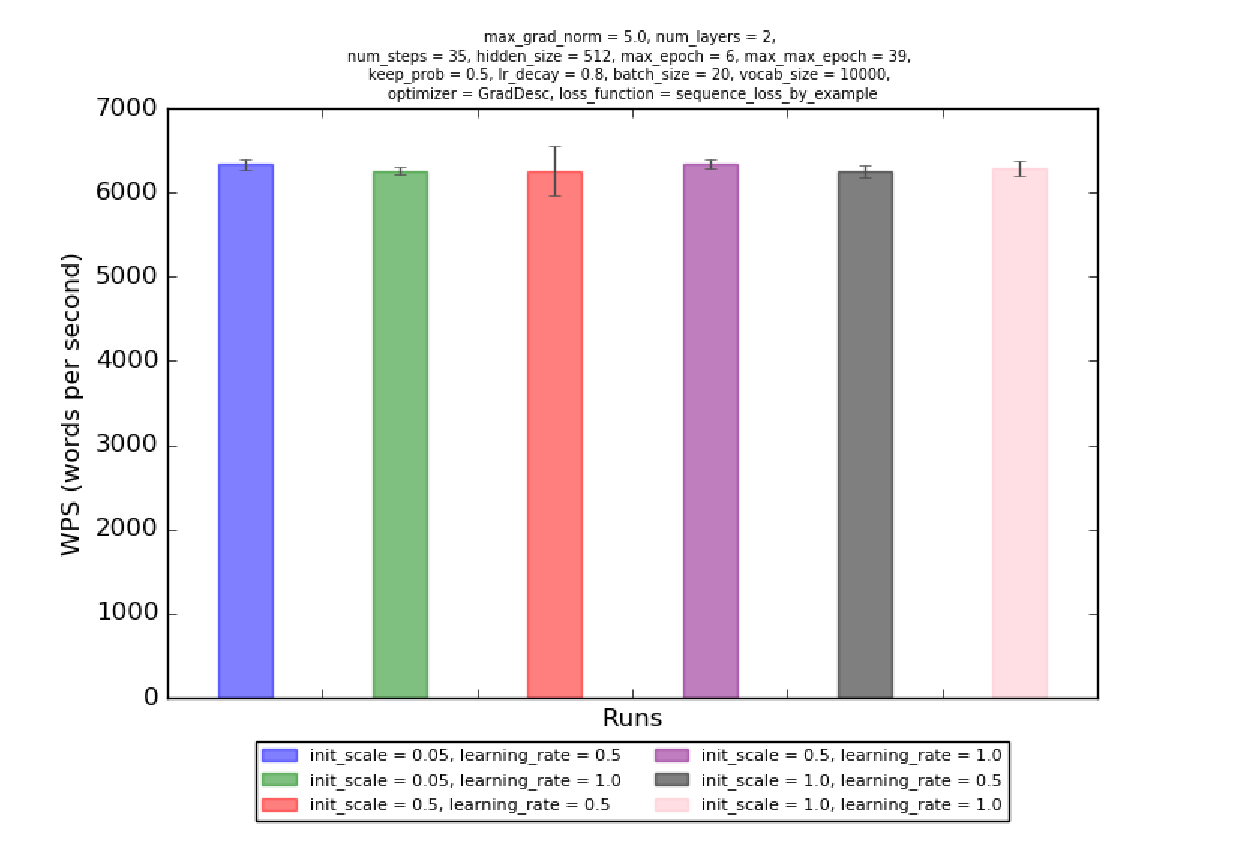
\includegraphics[width=0.72\textwidth]{initlearnspeed.eps}
		\caption{Results of speed experiment with \textbf{init\_scale \& learning\_rate} as variable parameters}
		\label{fig:exp2speed}
	\end{center}	
\end{figure}

\begin{figure}[H]
	\begin{center}
		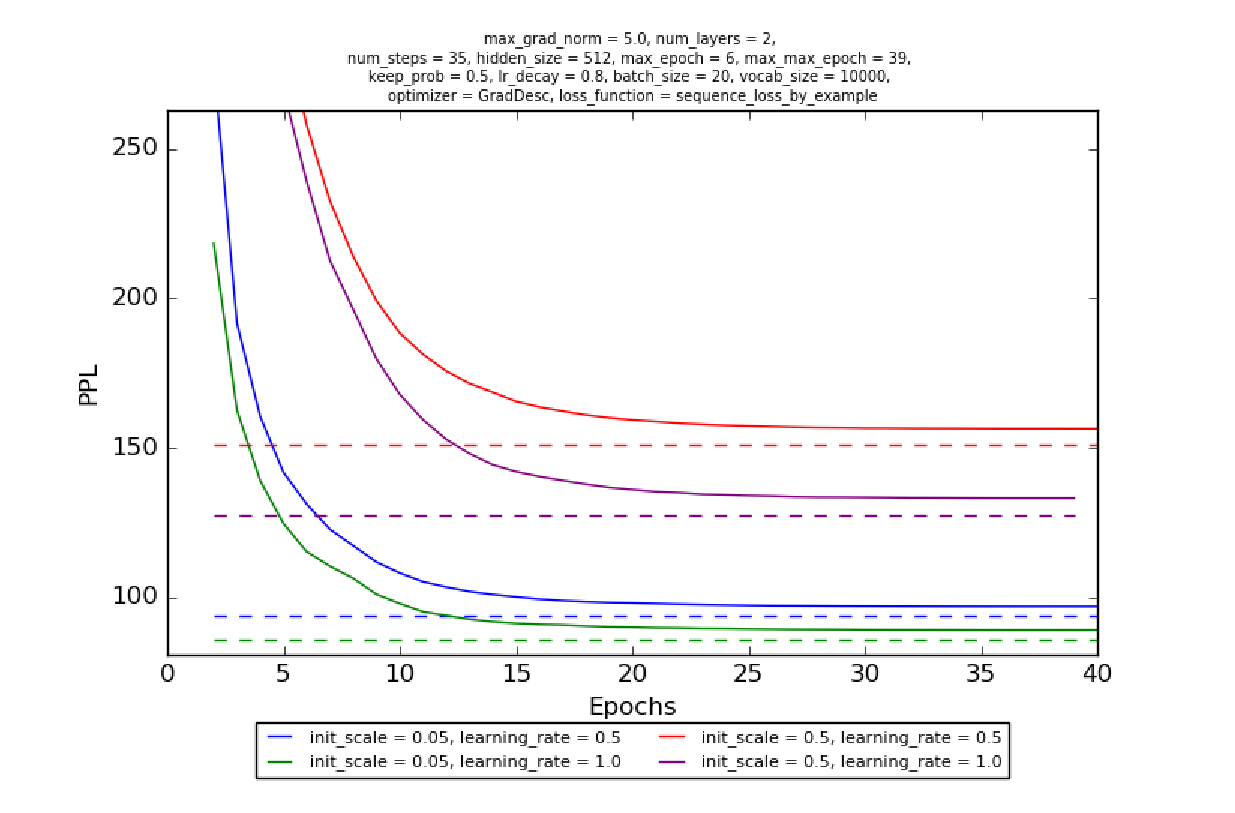
\includegraphics[width=0.72\textwidth]{initlearnperf.eps}
		\caption{Results of performance experiment with \textbf{init\_scale \& learning\_rate} as variable parameters. The full line represents the validation perplexity evaluated after each training epoch, the dotted line represent the test perplexity evaluated at the vary last epoch of the training.}
		\label{fig:exp2perf}
	\end{center}	
\end{figure}

The results of this experiment are displayed in figures \ref{fig:exp2speed} and \ref{fig:exp2perf}. Experiments with \textbf{init\_scale} equal to 1 were also performed but the performance results were so bad that these experiments are excluded from the figures. The results seem to suggest that it is beneficial to keep \textbf{init\_scale} fairly small and \textbf{learning\_rate} relatively large. The impact of the former also seems more significant than the impact of the latter.


\subsection{num\_steps \& batch\_size}

\begin{figure}[H]
	\begin{center}
		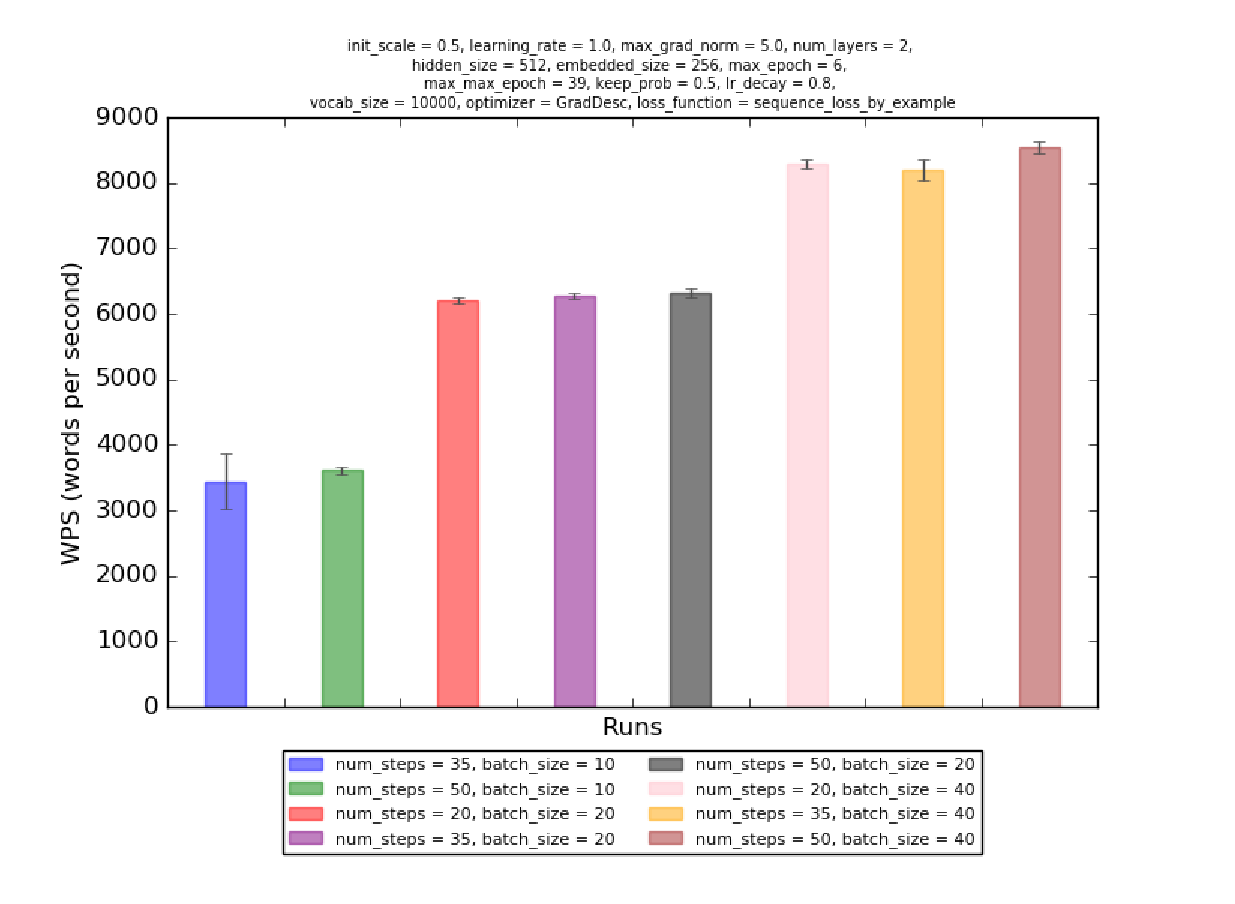
\includegraphics[width=0.72\textwidth]{stepsbatchspeed.eps}
		\caption{Results of speed experiment with \textbf{num\_steps \& batch\_size} as variable parameters}
		\label{fig:exp3speed}
	\end{center}	
\end{figure}

\begin{figure}[H]
	\begin{center}
		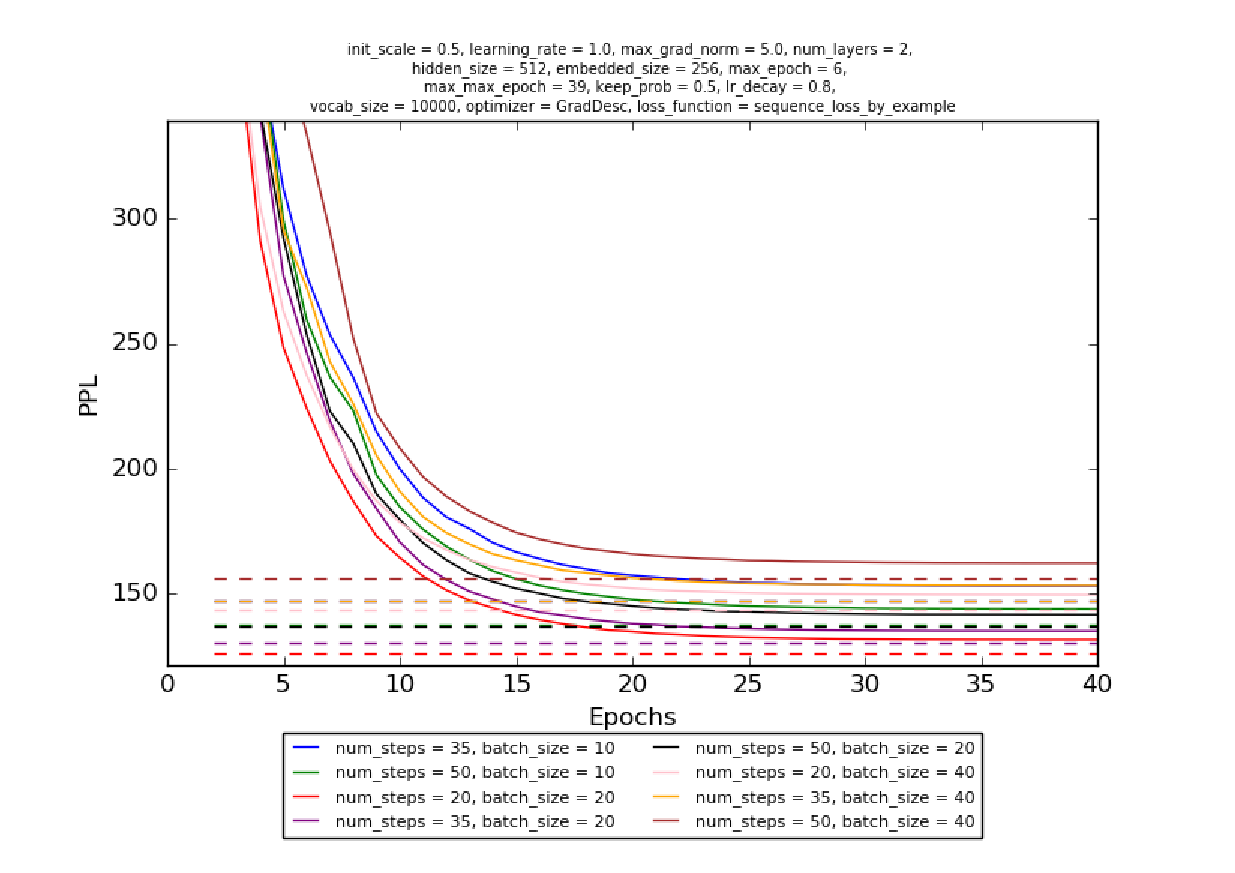
\includegraphics[width=0.72\textwidth]{stepsbatchperf.eps}
		\caption{Results of performance experiment with \textbf{num\_steps \& batch\_size} as variable parameters. The full line represents the validation perplexity evaluated after each training epoch, the dotted line represent the test perplexity evaluated at the vary last epoch of the training.}
		\label{fig:exp3perf}
	\end{center}	
\end{figure}

The results of this experiment are displayed in figures \ref{fig:exp3speed} and \ref{fig:exp3perf}. As expected,  as \textbf{batch\_size} goes up, the training speed slows down while there seems to be very little impact of \textbf{num\_steps} on the training speed. When it comes to the performance the results are much less clear: the best performing value for \textbf{batch\_size} is 20, in between 10 and 40, there seems to be a local optimum for this parameter. Regarding the parameter \textbf{num\_steps}, no definitive conclusion can be made based on this experiment.

\subsection{loss\_function}

\begin{figure}[H]
	\begin{center}
		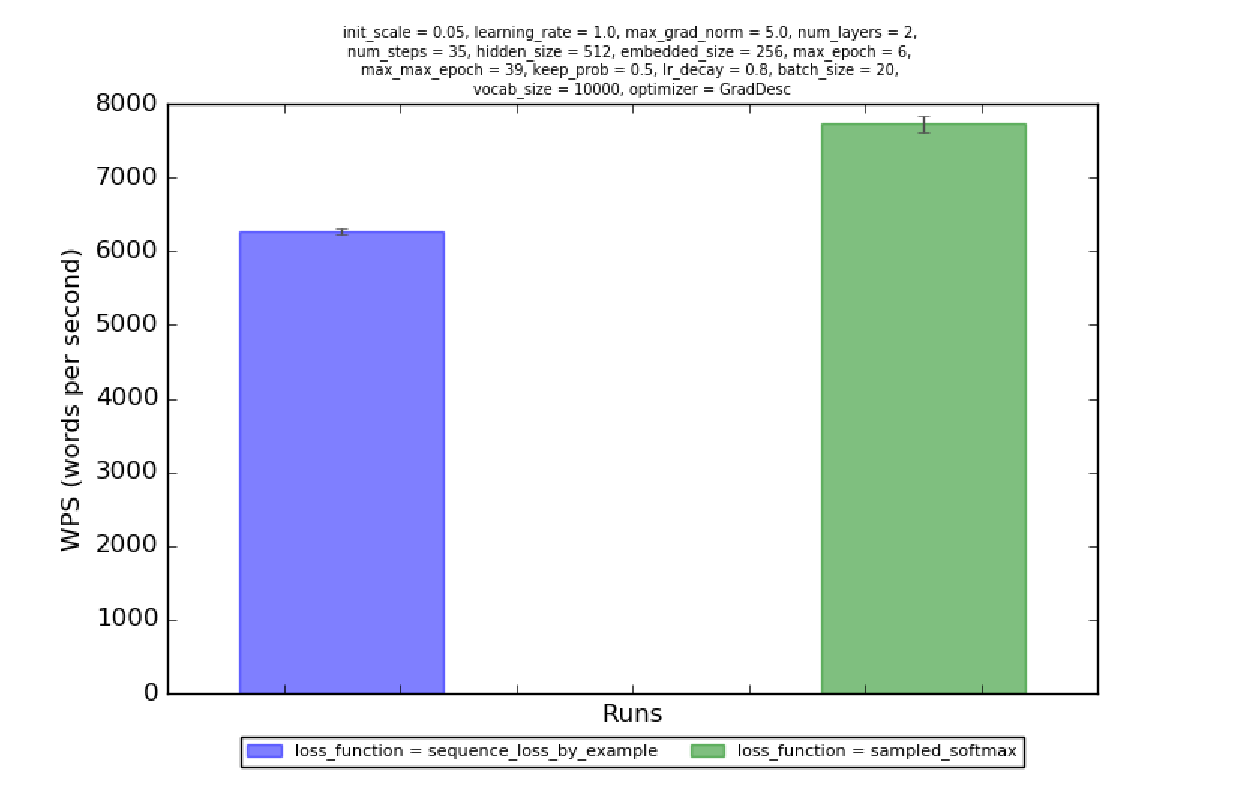
\includegraphics[width=0.72\textwidth]{lossspeed.eps}
		\caption{Results of speed experiment with \textbf{loss\_function} as variable parameters}
		\label{fig:exp4speed}
	\end{center}	
\end{figure}

\begin{figure}[H]
	\begin{center}
		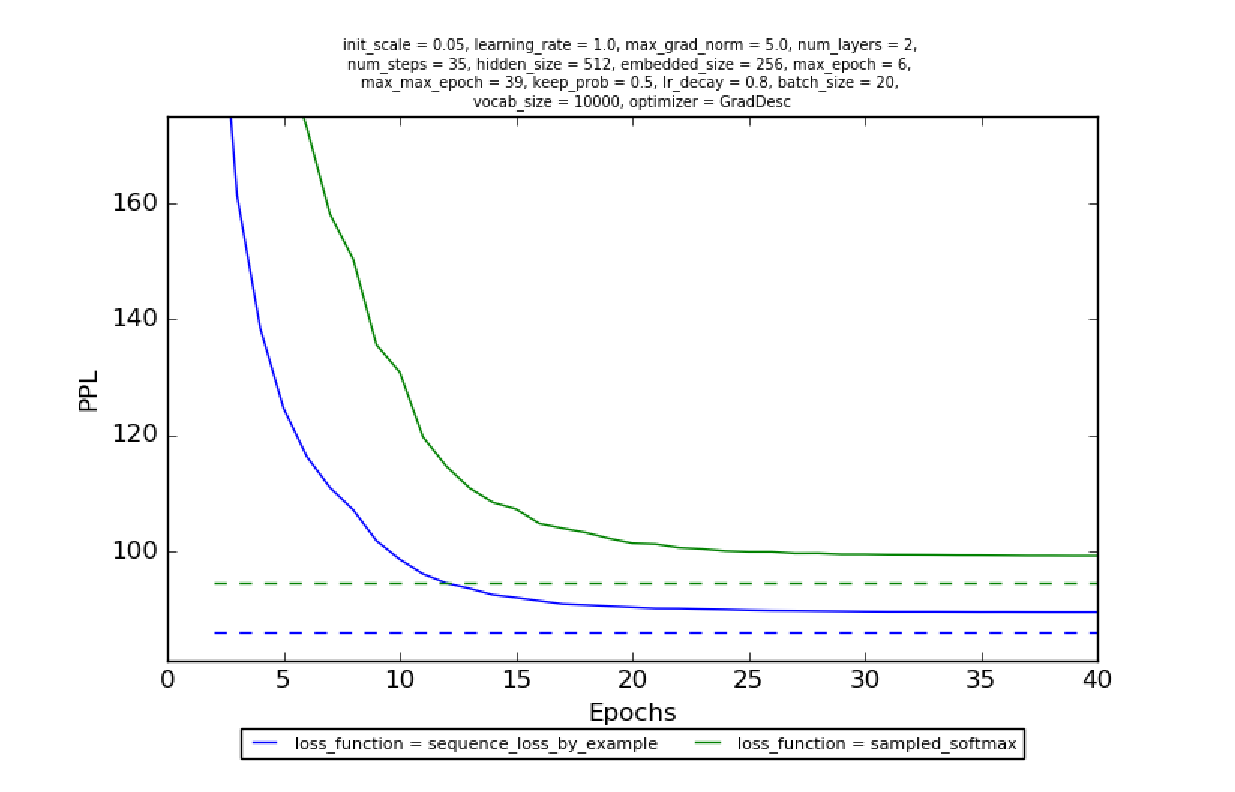
\includegraphics[width=0.72\textwidth]{lossperf.eps}
		\caption{Results of performance experiment with \textbf{loss\_function} as variable parameters. The full line represents the validation perplexity evaluated after each training epoch, the dotted line represent the test perplexity evaluated at the vary last epoch of the training.}
		\label{fig:exp4perf}
	\end{center}	
\end{figure}

The results of this experiment are displayed in figures \ref{fig:exp4speed} and \ref{fig:exp4perf}. The results are as expected, the sampled softmax loss function trains quicker but performs worse than the full softmax function. Extra experiments will have to be done to see if this loss in performance is worth the gain in speed

\subsection{optimizer}

\begin{figure}[H]
	\begin{center}
		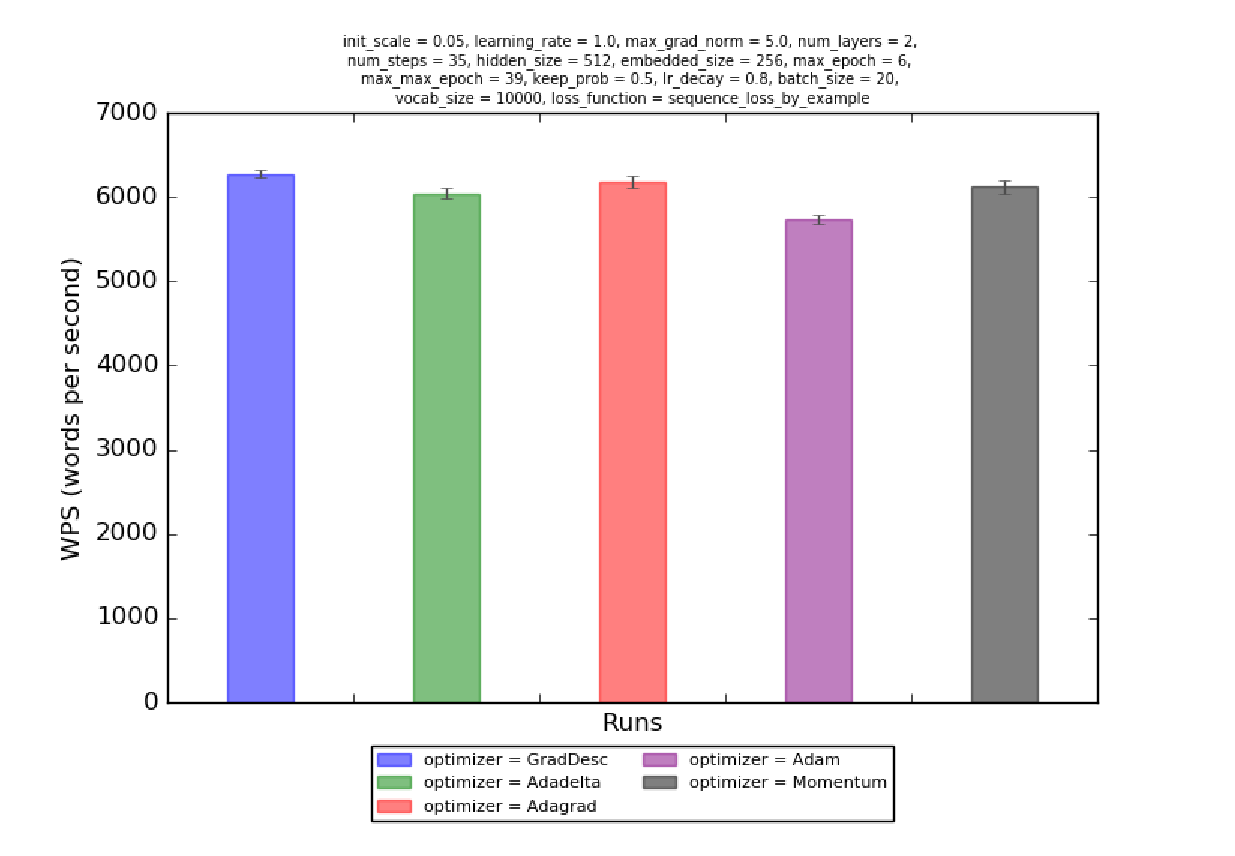
\includegraphics[width=0.72\textwidth]{optspeed.eps}
		\caption{Results of speed experiment with \textbf{optimizer} as variable parameters}
		\label{fig:exp5speed}
	\end{center}	
\end{figure}

\begin{figure}[H]
	\begin{center}
		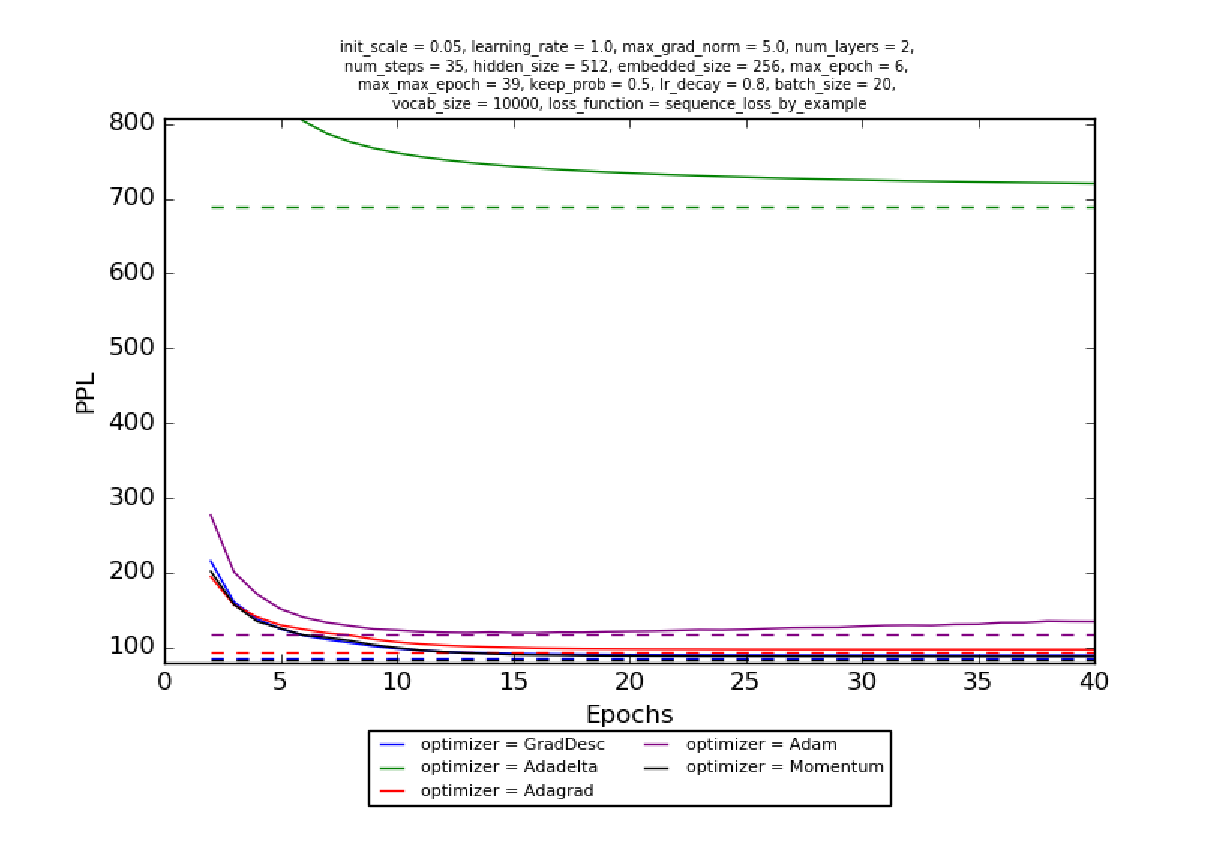
\includegraphics[width=0.72\textwidth]{optperf.eps}
		\caption{Results of performance experiment with \textbf{optimizer} as variable parameters. The full line represents the validation perplexity evaluated after each training epoch, the dotted line represent the test perplexity evaluated at the vary last epoch of the training.}
		\label{fig:exp5perf}
	\end{center}	
\end{figure}

The results of this experiment are displayed in figures \ref{fig:exp5speed} and \ref{fig:exp5perf}. There seems be one clear loser in this experiment: the Adadelta optimizing algorithm. The rest of the optimizing algorithms are close in terms of speed and performance. One special thing to note is that the Adam algorithm seems to suffer significantly from the fact that early stopping is not applied.

\subsection{num\_layers}

\begin{figure}[H]
	\begin{center}
		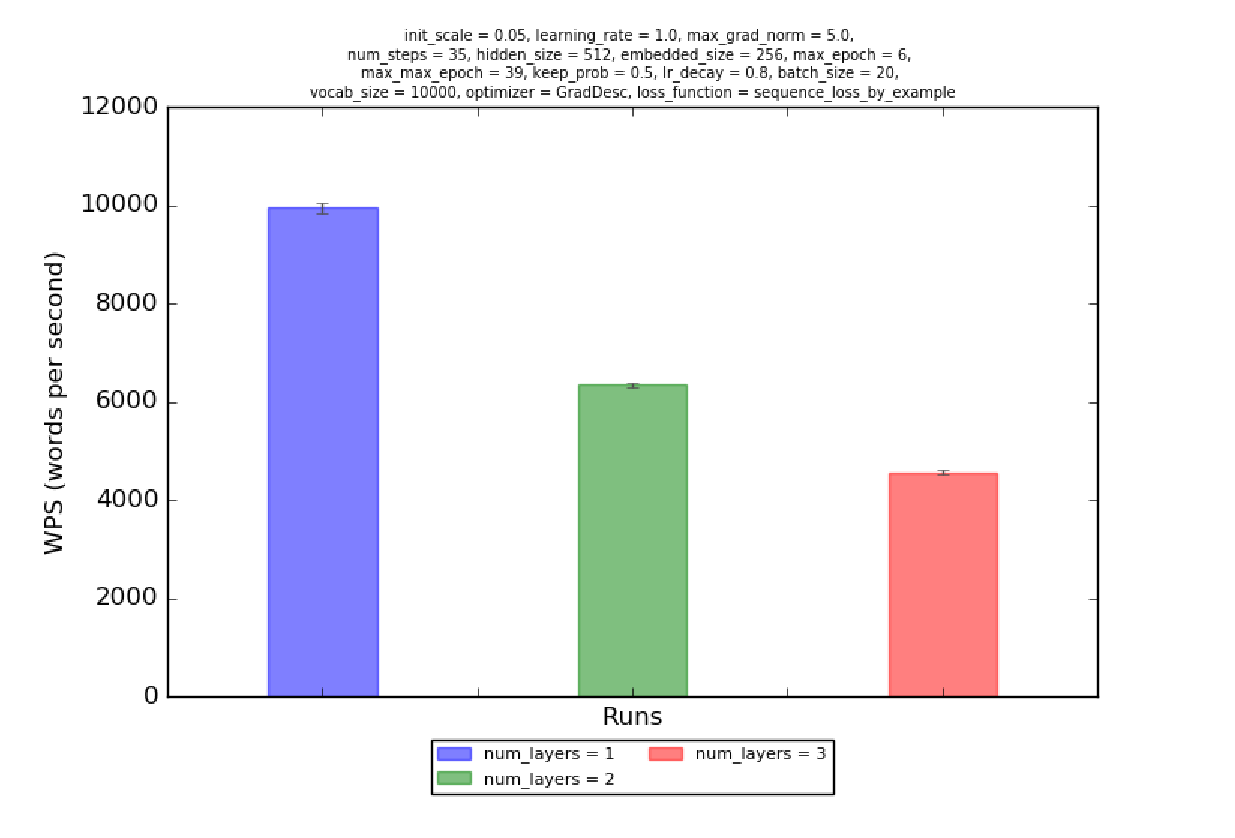
\includegraphics[width=0.72\textwidth]{layersspeed.eps}
		\caption{Results of speed experiment with \textbf{num\_layers} as variable parameters}
		\label{fig:exp6speed}
	\end{center}	
\end{figure}

\begin{figure}[H]
	\begin{center}
		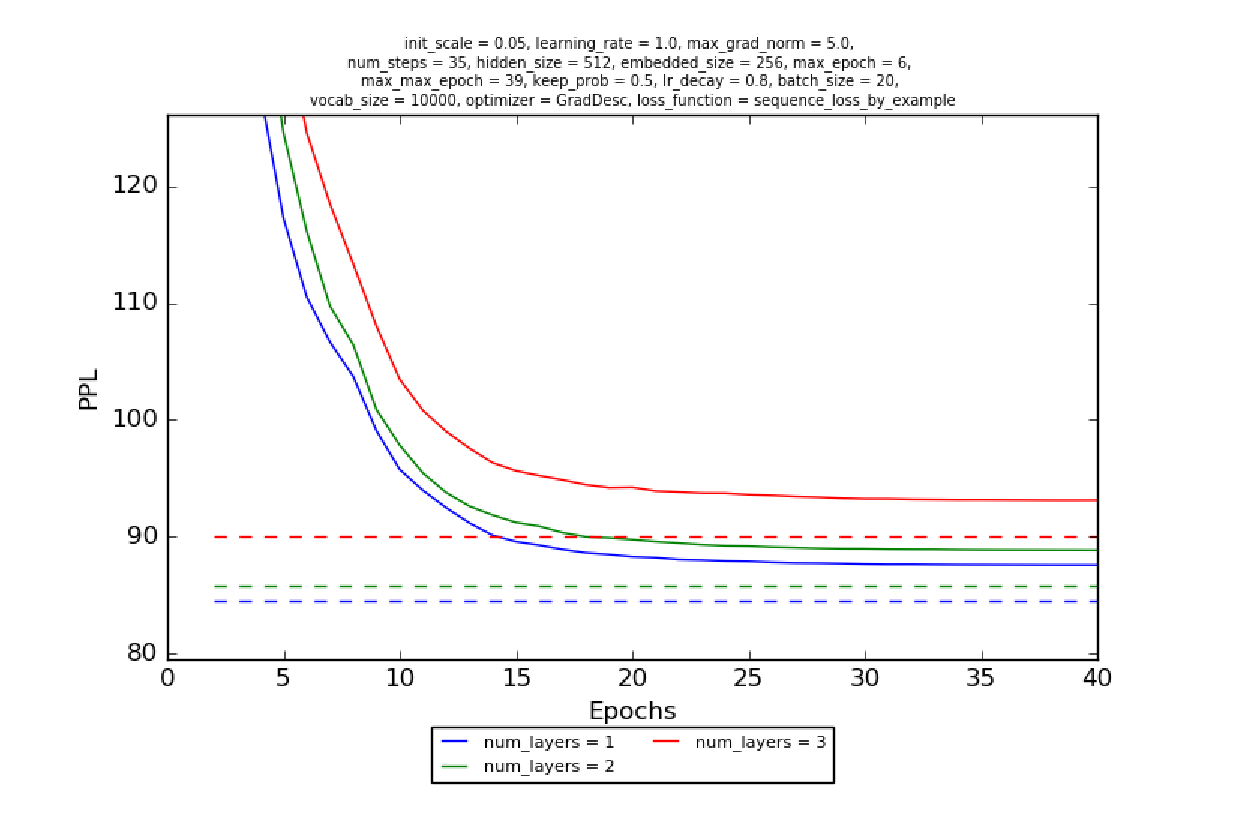
\includegraphics[width=0.72\textwidth]{layersperf.eps}
		\caption{Results of performance experiment with \textbf{num\_layers} as variable parameters. The full line represents the validation perplexity evaluated after each training epoch, the dotted line represent the test perplexity evaluated at the vary last epoch of the training.}
		\label{fig:exp6perf}
	\end{center}	
\end{figure}

The results of this experiment are displayed in figures \ref{fig:exp6speed} and \ref{fig:exp6perf}. The results seem to indicate that in this case it is better to stay away from multiple layers of LSTM cells. This could be because the number of model parameters (weights) increase heavily as \textbf{num\_layers} is increased, and there might not be enough training data available to cope with huge amounts of parameters.

\newpage
\section{Conclusion}

These experiments investigated the impact of the different training parameters involved when using recurrent neural networks for language modeling. To this end, the Tensorflow tutorial model of a recurrent neural network for language modeling (publicly available) was used with the Penn Tree Bank dataset for training, validation and testing of the model \cite{tensorflow}.\\
\\
The most interesting conclusions that could be drawn from these experiments are summarized in this list (see section \ref{subsec:exp} for an explanation of the parameters):

\begin{itemize}
	\item Increasing \textbf{hidden\_size} improves performance but lowers training speed.
	\item Increasing \textbf{embedded\_size} improves performance slightly but does not have an impact or very little impact on training speed.
	\item \textbf{init\_scale} should be kept at a relatively low value.	
	\item \textbf{learning\_rate} should be kept at a relatively high value.
	\item The parameter \textbf{batch\_size} seems to have a local optimum regarding performance.
	\item No real conclusions could be drawn from these experiments regarding \textbf{num\_steps}. 
	\item The sampled softmax loss function has worse performance but better training speed than the full softmax loss function. 
	\item Most optimizing algorithms are relatively close in performance besides Adadelta, that performs much worse than the other options.
	\item The optimal value for \textbf{num\_layers} in this case is 1. However, this could be because there is not enough training data to properly train the model when multiple LSTM layers are employed.
\end{itemize}

\newpage
\addcontentsline{toc}{section}{References}
\begin{thebibliography}{9}
	
	\bibitem{tensorflow}
	\textit{https://www.tensorflow.org/versions/r0.11/tutorials/recurrent/index.html}
	
	\bibitem{LSTM}
	\textit{http://colah.github.io/posts/2015-08-Understanding-LSTMs/}
	
	\bibitem{PTB}
	\textit{http://www.cis.upenn.edu/~treebank/home.html}
	
	\bibitem{dropout}
	\textit{https://www.cs.toronto.edu/~hinton/absps/JMLRdropout.pdf}
	
	\bibitem{opt}
	\textit{https://www.tensorflow.org/versions/r0.11/api\_docs/python/train.html}
	
	\bibitem{bptt}
	\textit{http://ir.hit.edu.cn/~jguo/docs/notes/bptt.pdf}
	
	\bibitem{exp}
	\textit{http://www.wildml.com/2015/10/recurrent-neural-networks-tutorial-part-3-backpropagation-through-time-and-vanishing-gradients/}
	
	\bibitem{cross}
	\textit{http://homes.esat.kuleuven.be/~jpeleman/wim\_en\_robbe/jurafsky04.pdf}
	
	\bibitem{sampled}
	\textit{https://arxiv.org/pdf/1412.2007v2.pdf}
	
\end{thebibliography}
	
\end{document}